\documentclass{beamer}

\usepackage[beamer]{shortcut}
\usepackage{bibentry}

\graphicspath{{./images/}}
\usepackage[square]{natbib}



\newcommand{\rightcite}[1]{\keypoint{\small[{\color{linkcolor} #1}]}}
\newcommand{\bottomlink}[1]{\vspace{0pt plus 1 filll}\rightcite{#1}}

\newcommand{\techterm}[1]{
	\column{\widthof{\bf #1g}}
    \centering
    \begin{beamercolorbox}[rounded=true, shadow=true]{title}%
        {\centering\bf #1\hskip-1ex\phantom{g}\\}
    \end{beamercolorbox}%
}

\newcommand{\highlightbox}[1]{
    \begin{beamercolorbox}[rounded=true,
                           shadow=true]{title}
        #1
    \end{beamercolorbox}}


\def\keypoint#1{\hspace{0pt plus 1 filll}\textcolor{gray}{#1}}
\def\mycite#1{\keypoint{\small\citep{#1}}}
\def\tT{\widetilde{T}}

\institute{\\ INRIA Saclay}
\author{Thomas Moreau}
\title{
	Multivariate Convolutional Sparse Coding for Electromagnetic Brain Signals}

\date{
	May 29, 2018
}

\setbeamertemplate{title page}[frame]
\def\extraLogo{}
\collaborators{Dupré La Tour T., Mainak J., Gramfort A.}

\begin{document}

\begin{frame}
	\titlepage
    \nobibliography{../../library}
\end{frame}



\frame{
    \frametitle{Context: Functional Neuroimaging}

    \large {\bf Goal:}
    Study the brain mechanisms while it is functioning.\\[1em]

    {\bf Outputs:}\\[.3em]
    \begin{itemize}\itemsep1em
        \item {\bf Functional Atlases:} Link areas of the brain to specific cognitive functions.
        \item {\bf Functional Connectivity:} Highlight the information flow in the brain.
        \item {\bf Healthcare:} Develop bio-markers for neurological disorders.
        \item \dots
    \end{itemize}
}

\frame[t]{
    \frametitle{Context: Functional Neuroimaging}

    {\large How to record living brains activity: \textbf{Electrophysiology}}\\[.3em]

    \centering\large Direct measurement of electrical activity.\\[.5em]
        \centering
        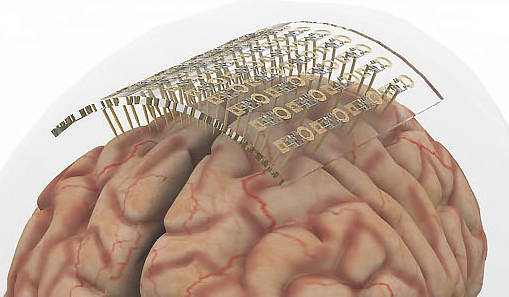
\includegraphics[width=.7\textwidth]{brain_probe.jpg}\\[1em]
        \begin{columns}
            \techterm{\color{darkblue} High Localization}%
            \techterm{Low Resolution}%
            \techterm{Invasive}%
        \end{columns}
}

\frame[t]{
    \frametitle{Context: functional Neuroimaging}

    {\large How to record living brains activity: \textbf{Electrophysiology}}\\[.3em]

    \large\centering Remote measurement of the electrical activity.\\[-.5em]
    \begin{columns}[T]
        \column{.35\textwidth}
        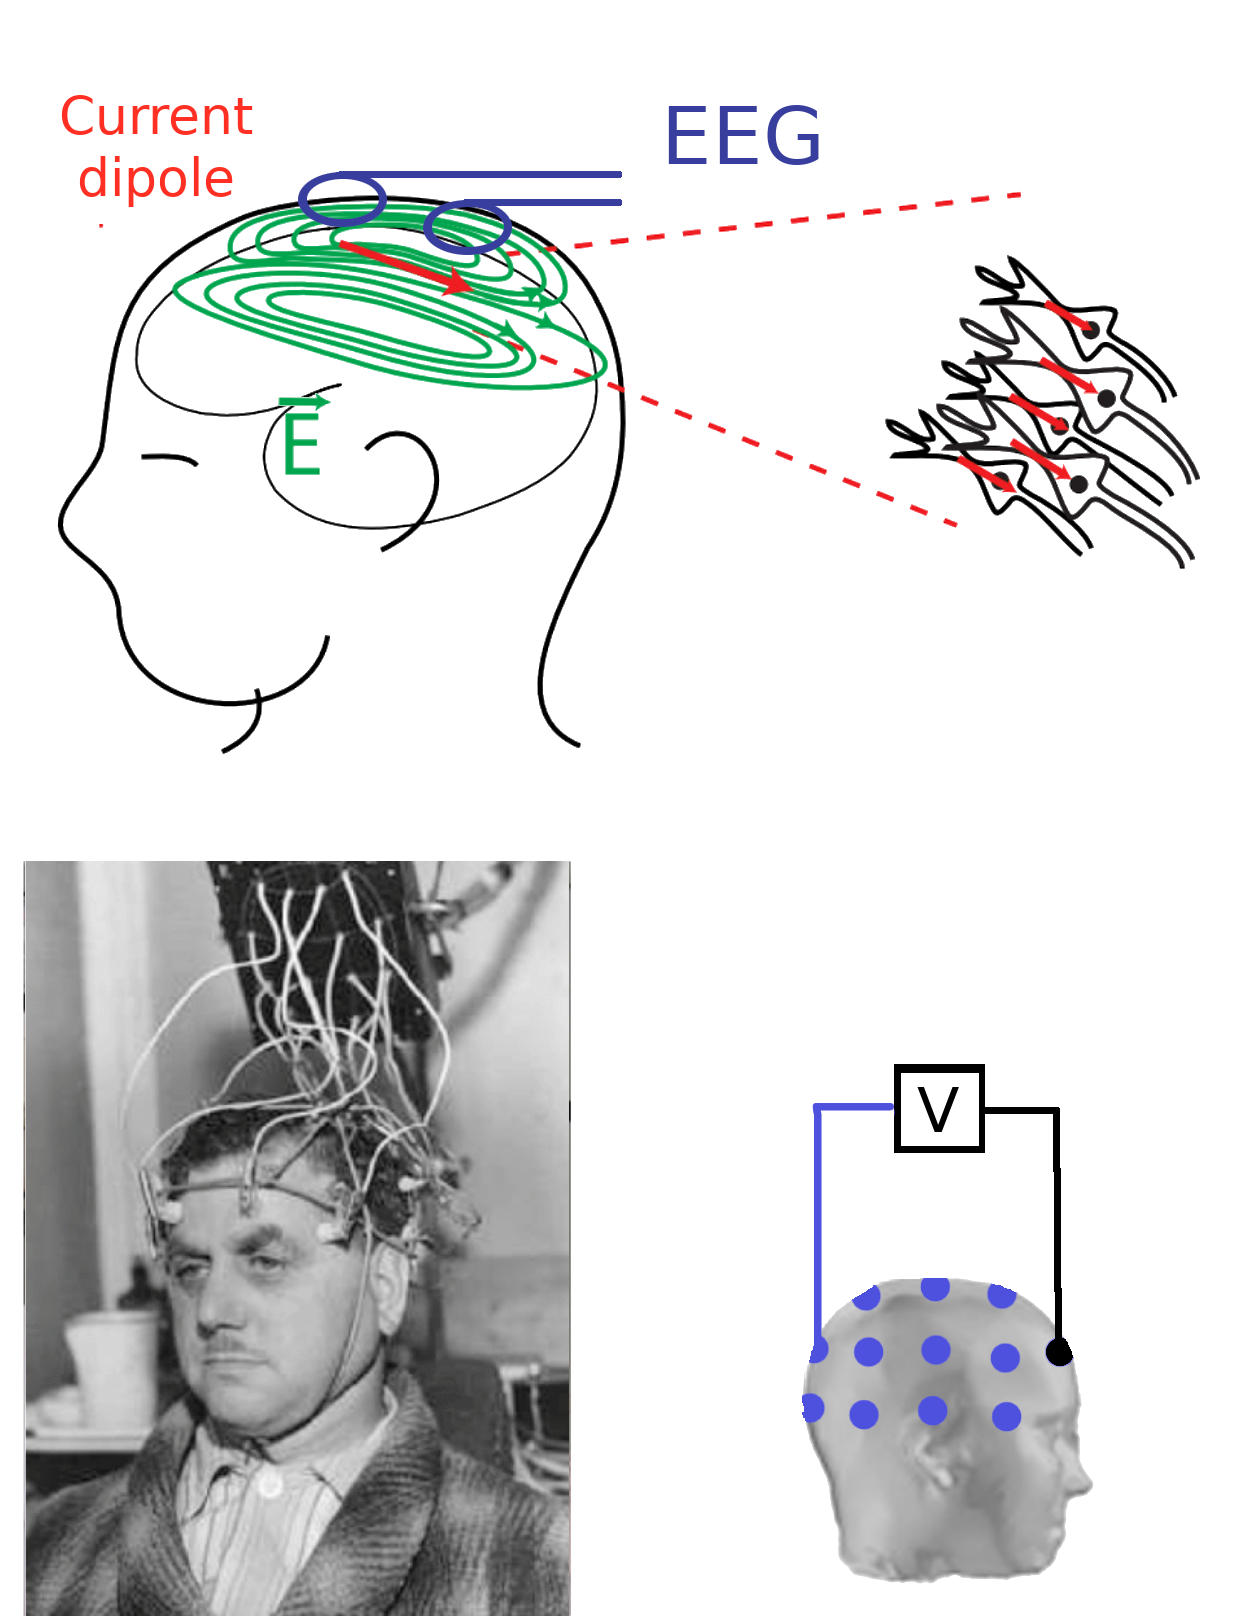
\includegraphics[width=\textwidth]{eeg_presentation}
        \column{.35\textwidth}
        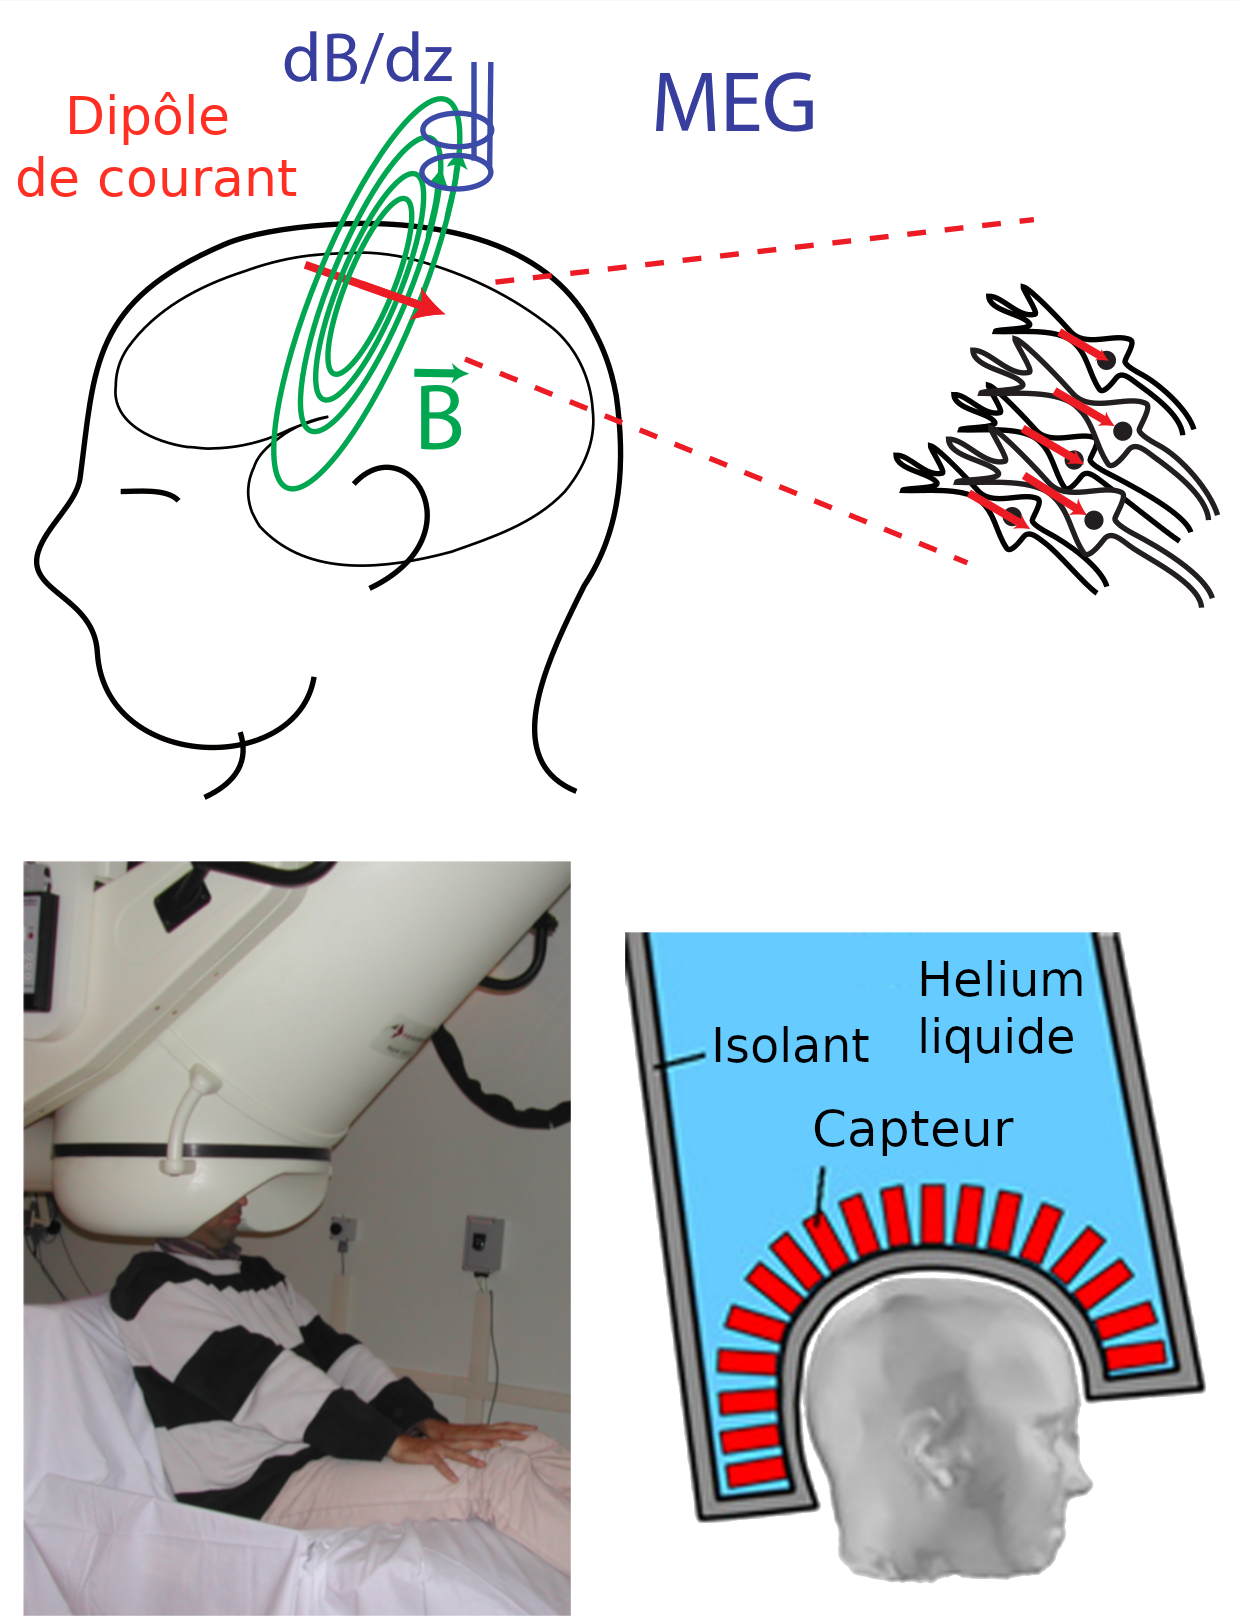
\includegraphics[width=\textwidth]{meg_presentation}
    \end{columns}
    % \only<2>{
    \begin{columns}
        \techterm{No Localization}%
        \techterm{\color{darkblue} Global}%
        \techterm{\color{darkblue} Non Invasive}%
    \end{columns}
    % }

}



\frame{
    \frametitle{}

    \begin{columns}[c]
        \column{.6\columnwidth}
    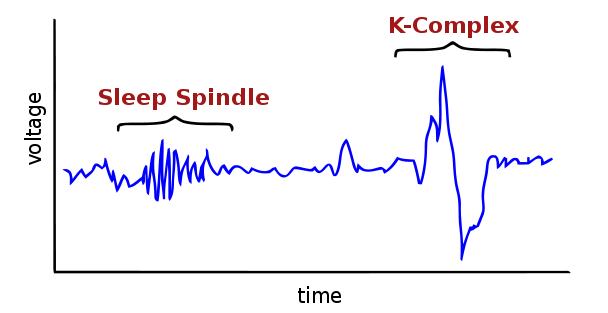
\includegraphics[width=\textwidth, trim={6em 6em 0 0}, clip]{sleep_spinddle}
        \column{.35\columnwidth}
        \visible<2->{
            \highlightbox{
                \centering \Large
                Neural signals exhibit
                diverse and complex
                morphologies
            }
        }
    \end{columns}
    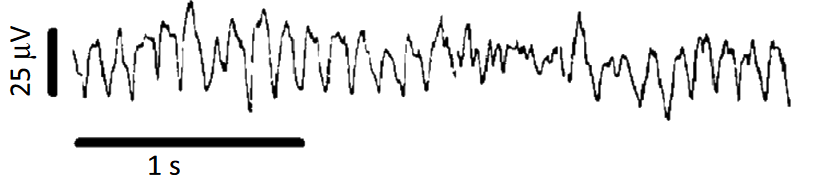
\includegraphics[width=\textwidth]{mu_rythm}\\[-1.5em]
    \rightcite{S. Cole, B. Voytek (2017) Trends in Cognitive Sciences}
    \vskip-7em
        \begin{columns}[c]
        \column{.75\columnwidth}
        \visible<3->{\highlightbox{\vskip.1em
        \Large Waveform shape can be related to diseases\\
        \eg{} Parkinson \rightcite{Jackson et al. (2019)}}\\[.3em]}
        \end{columns}
    \vskip3em
    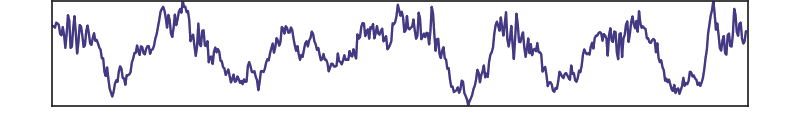
\includegraphics[width=\textwidth]{cfc}\\[-.8em]
    \rightcite{\footnotesize Dupré la Tour, Tallot, Grabot, Doyère, van Wassenhove, Grenier, Gramfort\\
    \hfill (2017) PLOS Computational biology}
}

\frame{
        \frametitle{"Textbook" brain rythm}

        \centering
        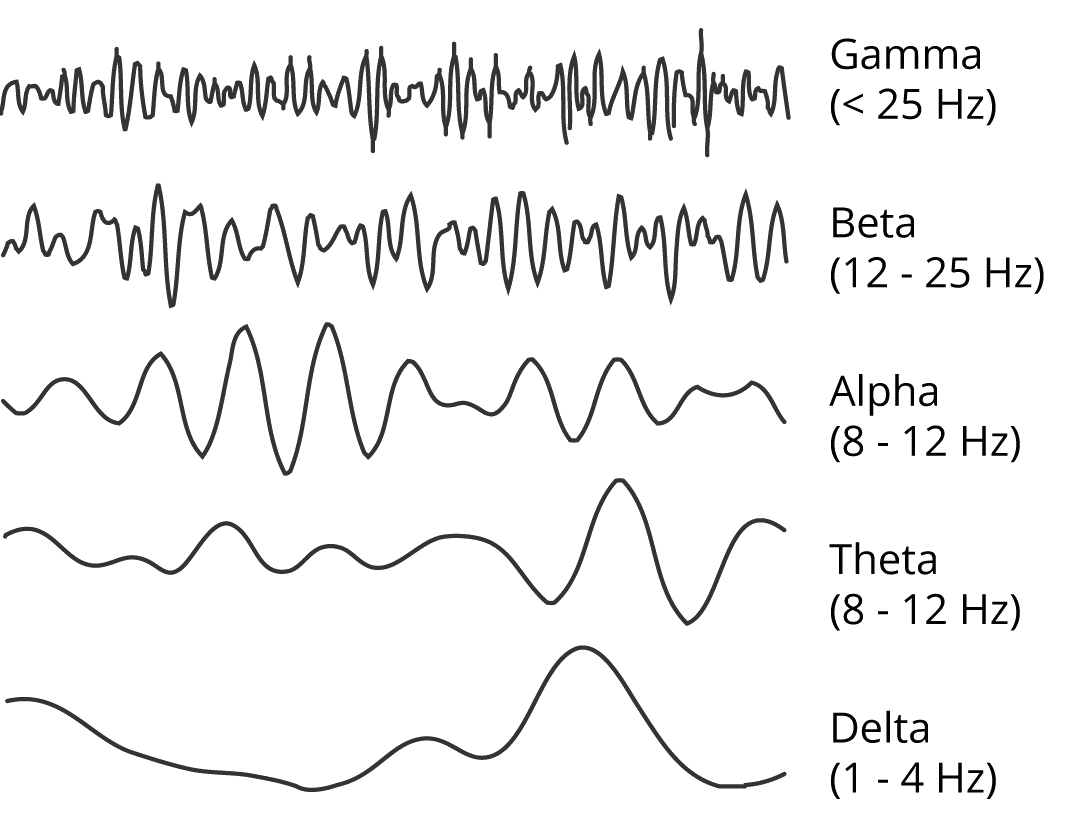
\includegraphics[width=.8\textwidth]{brain_rythm}

}


\frame{
    \frametitle{Linear filtering}

    After Linear filters, everything looks like a sinusoïd.
    {\centering
    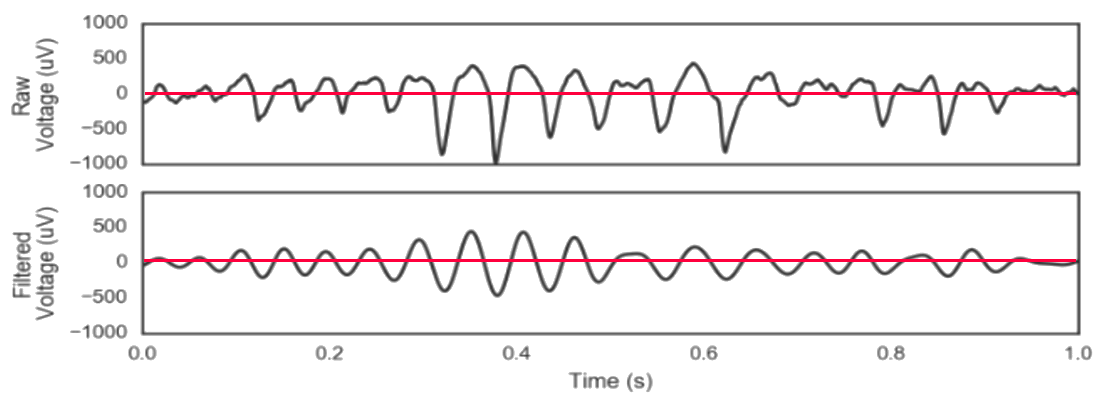
\includegraphics[width=.9\columnwidth]{filtering_mu_waves}\\[1em]
    $\Rightarrow$ Lose the asymmetry and the shape information.
    }

}

\frame{
    \frametitle{Fourier Fallacy}
    \large
    {\centering
    "Even though it may be possible to analyze the complex forms of brain waves into a {\bf number of different sine-wave} frequencies, this may lead only to what might be termed a “{\bf Fourier fallacy}”, if one assumes {\bf ad hoc} that all of the necessary frequencies actually occur as periodic phenomena in {\bf cell groups} within the brain."\\[.5em]}
    \rightcite{Jasper (1948)}
    \vskip.5em
    \visible<2->{
        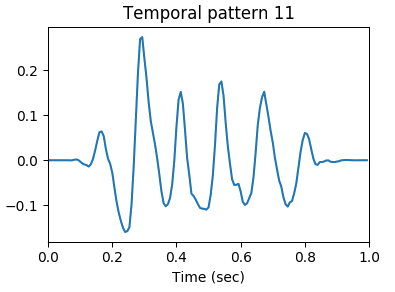
\includegraphics[width=.5\textwidth]{mu_waveform}%
        \alt<3>{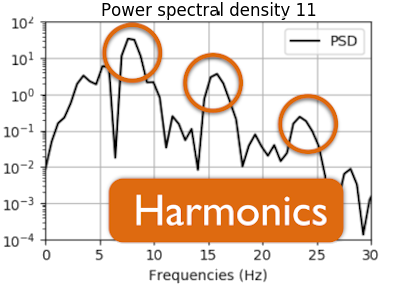
\includegraphics[width=.5\textwidth]{mu_waveform_harmonic}}
               {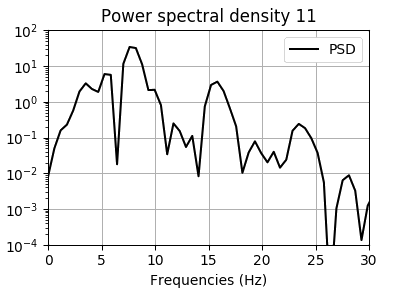
\includegraphics[width=.5\textwidth]{mu_waveform_psd}}
    }

}

\section{Learning the waveform:\\Convolutional Dictionary Learning}
\parttitleframe{Grosse2007}

\frame[t]{
	\frametitle{Local structure in signals}

	\visible<5->{
		\textbf{Key idea}: decouple the localization of the
							patterns and their shape}
    \vskip.5em%
    \centering%
    \only<1>{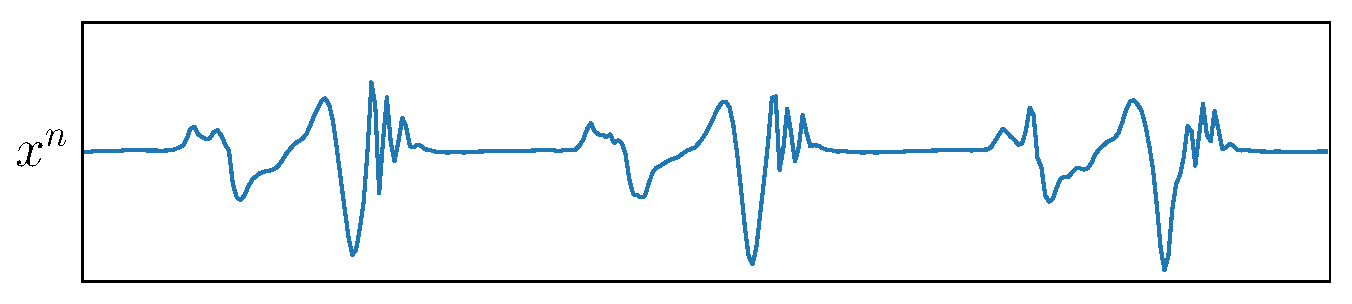
\includegraphics[width=\textwidth]{intro_csc_0}}%
    \only<2>{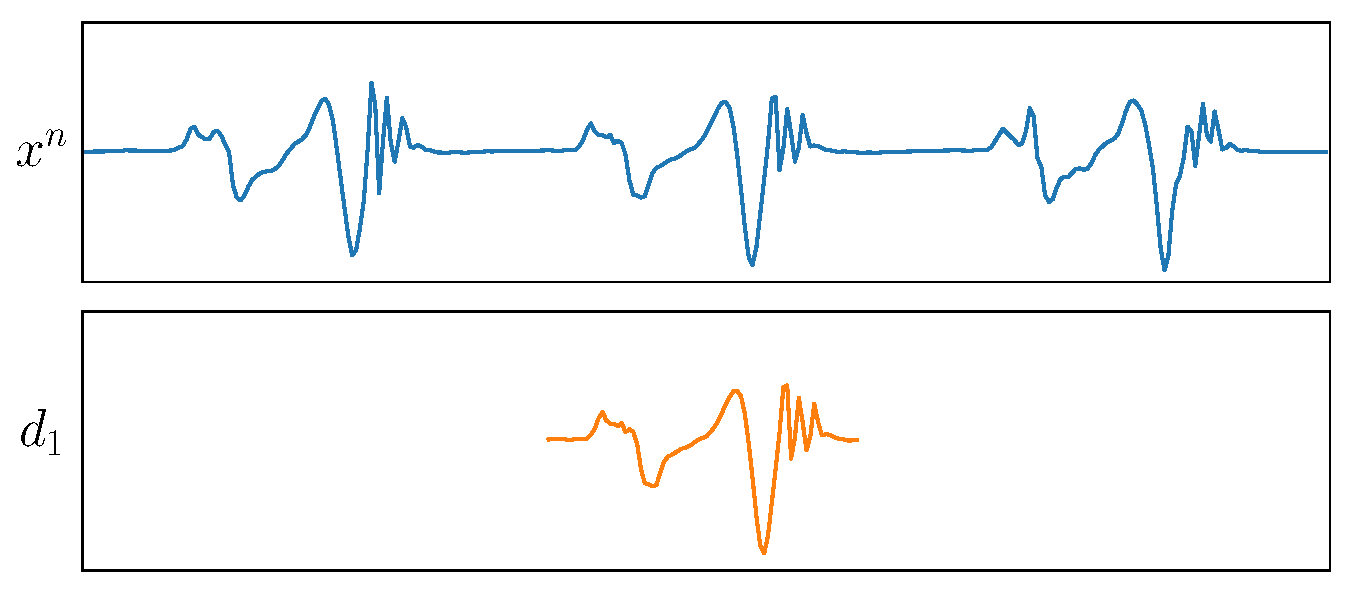
\includegraphics[width=\textwidth]{intro_csc_1}}%
    \only<3>{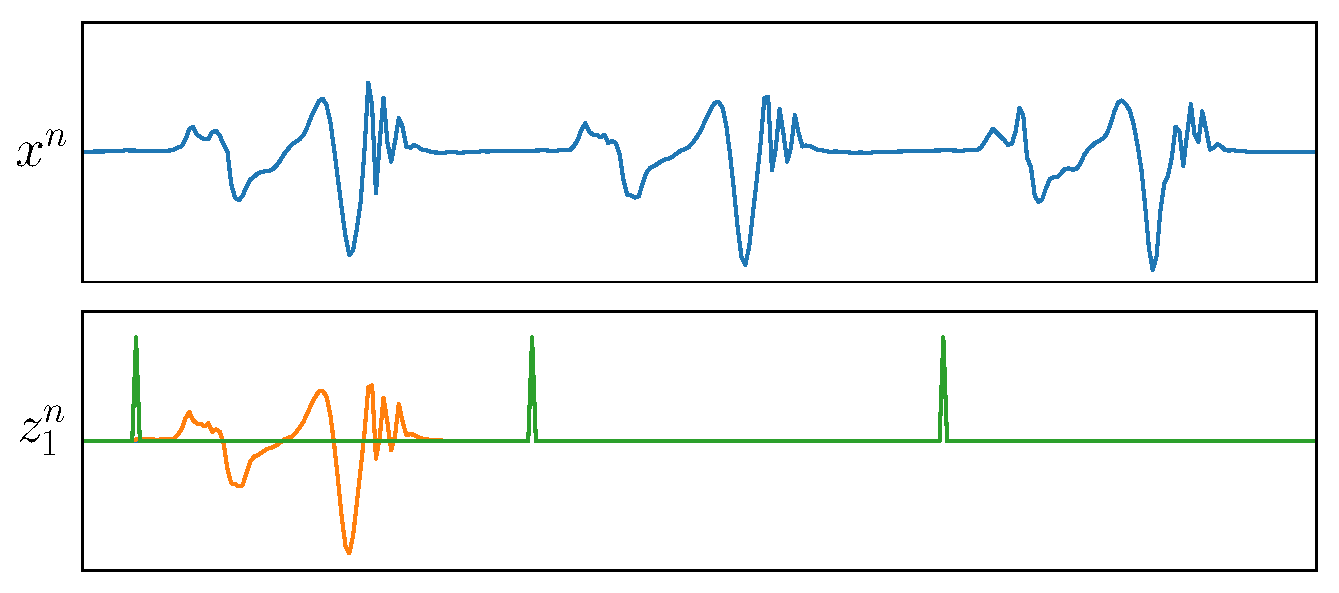
\includegraphics[width=\textwidth]{intro_csc_2}}%
    \only<4>{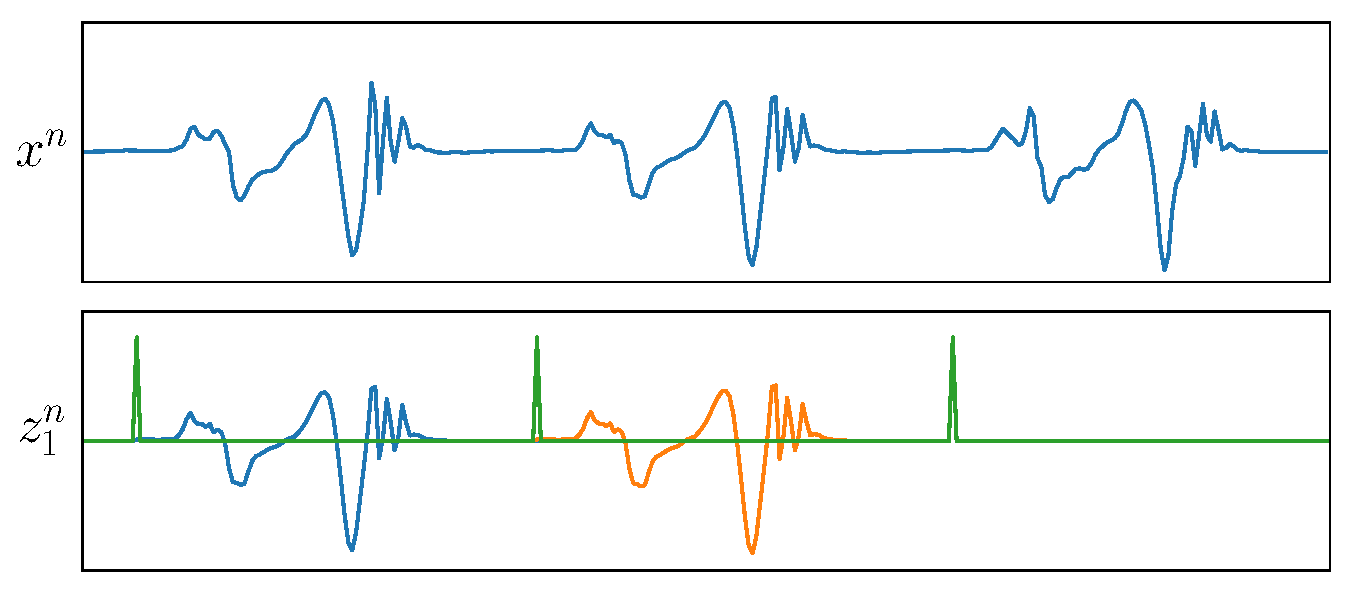
\includegraphics[width=\textwidth]{intro_csc_3}}%
    \only<5>{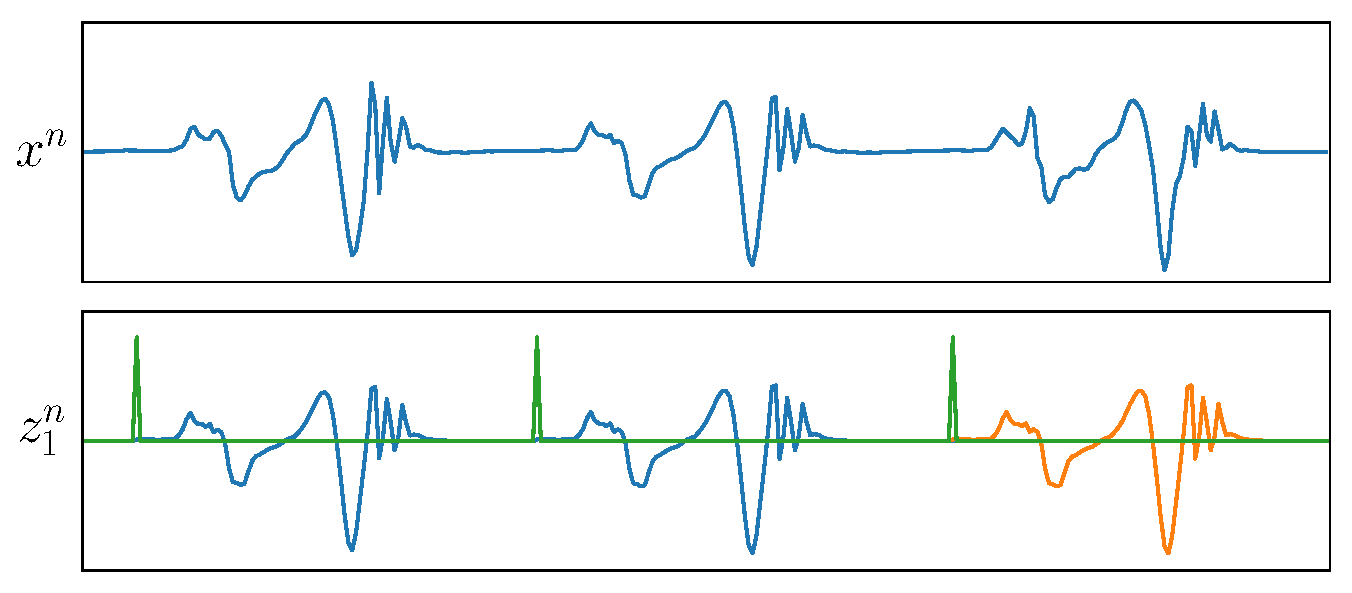
\includegraphics[width=\textwidth]{intro_csc_4}}%
    \only<6->{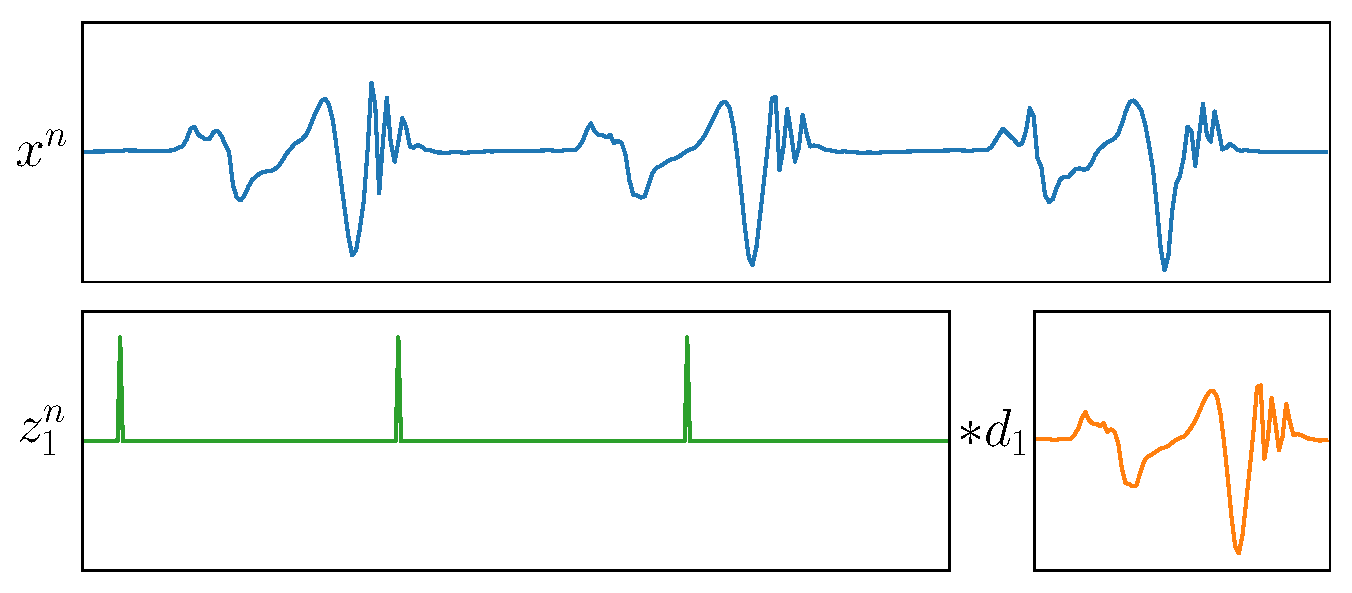
\includegraphics[width=\textwidth]{intro_csc_5}}%
    \vskip0em%
    \only<7>{%
        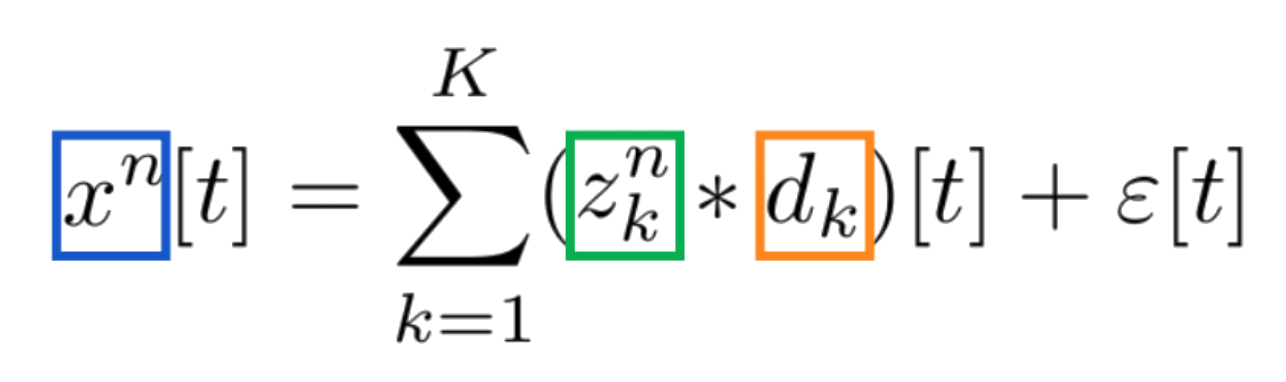
\includegraphics[width=.6\textwidth]{csc_explain_eq_color}%
    }
}

\frame{
    \frametitle{Convolutional Dictionary Learning \rightcite{Grosse2007}}

    For a set of $N$ univariate signals $x^n$, solve\\[.5em]
        {\centering 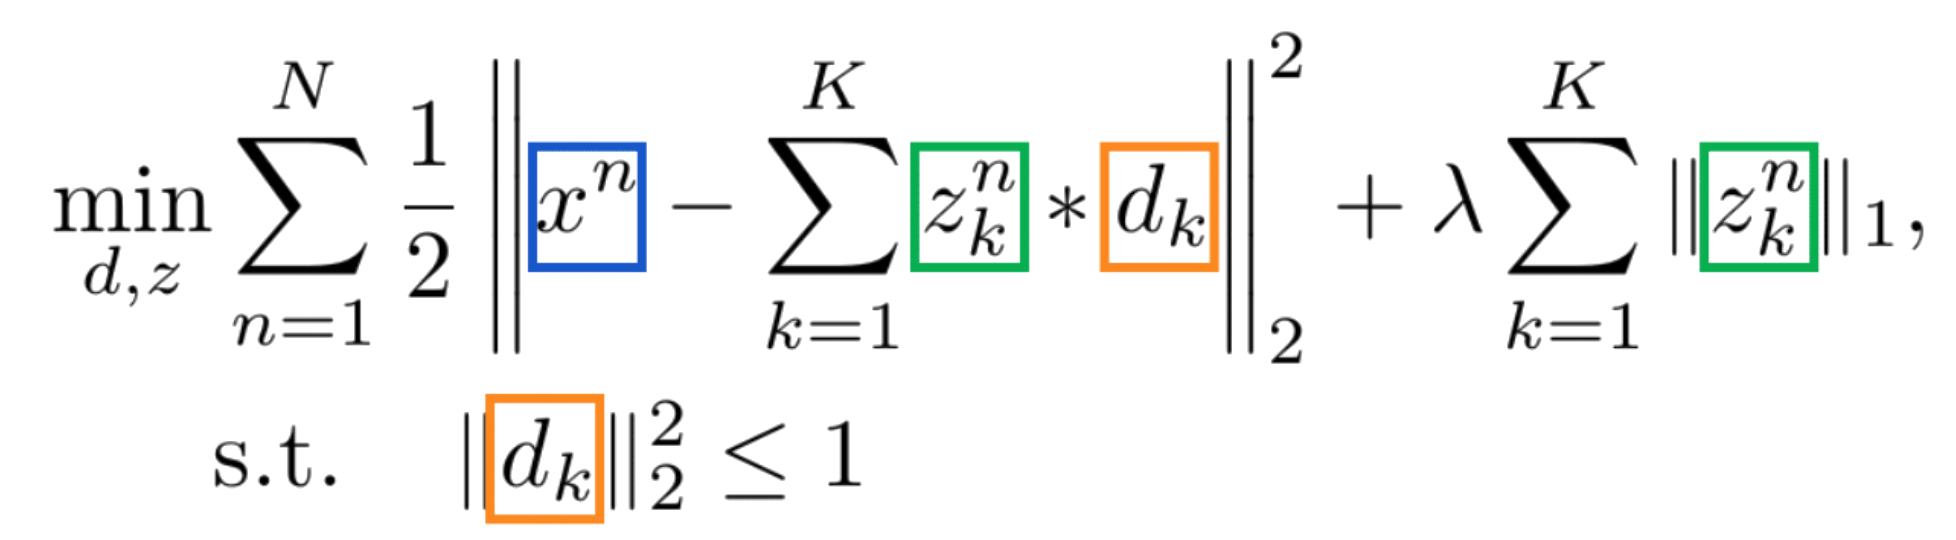
\includegraphics[width=.8\textwidth]{csc_eq_l1}\\[1em]}
    \textbf{Hypothesis:} patterns $d_k$ are not present everywhere in the signal. They are localized in time.
    \strongpoint{Sparse activation signals $z$}
    \vskip2em
    \textbf{Technical hypothesis:} the patterns are in the $\ell_2$-ball: $\|d_k\|_2^2 \le 1$.
}

\frame{
    \frametitle{Optimization strategy}
    \textbf{Bi-convex:} The problem is not jointly convex in $z^n_k$, and  $d_k$
    but it is convex in each block of coordinate.\\[1em]

    \textbf{Alternate minimization} (\emph{a.k.a.} Bloc Coordinate Descent):\\[.5em]

    \begin{itemize}\itemsep1em
    \item \textbf{Z-step:} given a fixed estimate of the atom, compute the activation signal $z^n_k$ associated to each signal $x^n$.
    \item \textbf{D-step:} given a fixed estimate of the activation, update the atoms in the dictionary $d_k$.
    \end{itemize}
}


\frame{
    \frametitle{Learned atoms \rightcite{Jas et al. (2017)}}
    \begin{columns}[T]
        \column{.2\columnwidth}
            \flushright \Large Data:
        \column{.8\columnwidth}
            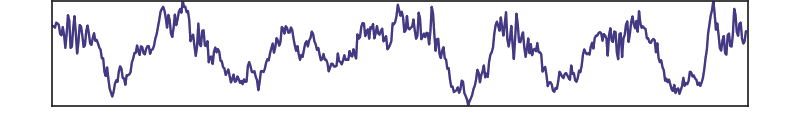
\includegraphics[width=\columnwidth]{cfc}
    \end{columns}
    \begin{columns}[c]
        \column{.5\columnwidth}
            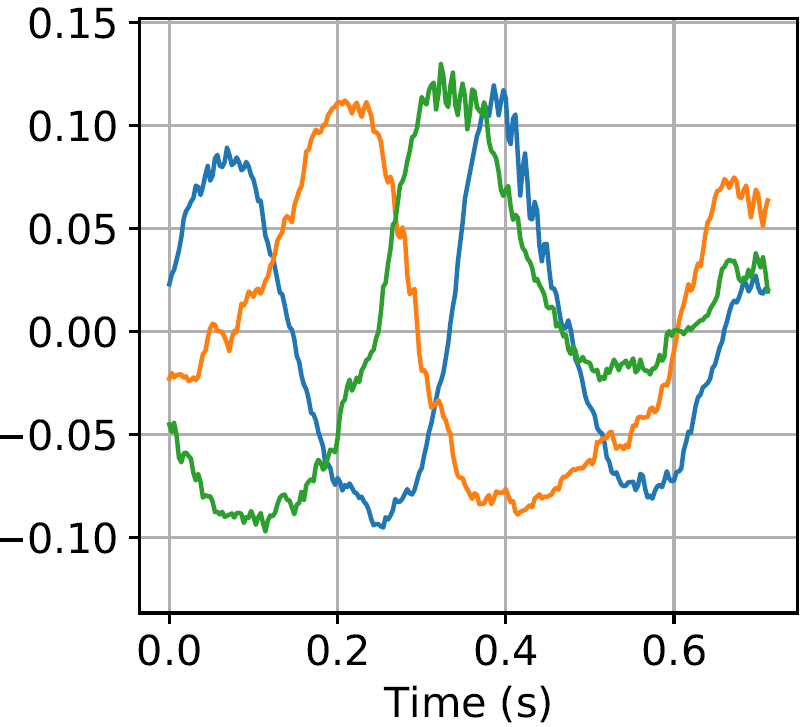
\includegraphics[width=\columnwidth]{learned_cfc}
        \column{.1\columnwidth}
        \column{.3\columnwidth}
            \visible<2>{
            \highlightbox{
                \centering
                \Large What to do\\in the case of\\multivariate signals?
            }}
        \column{.1\columnwidth}


    \end{columns}
}


\begin{frame}{How to extend CSC to multivariate signals?}
    We can just use multivariate convolution,
    \[
        \underbrace{X[t]}_{\in\Rset^P} = \sum_{k=1}^K \left(z_k * D_k\right)[t] = \sum_{k=1}^K \sum_{\tau=1}^L z_k[t-\tau] \underbrace{D_k[\tau]}_{\in \Rset^P}
    \]
    with:
    \begin{itemize}
        \item $X$ a multivariate signal of length $T$ in $\Rset^P$
        \item $D_k$ a multivariate signal of length $L$ in $\Rset^P$
        \item $z_k$ a univariate activation signal of length $\tT = T - L + 1$
    \end{itemize}
    \vskip1em
    However, this model does not account for the physics of the problem.
    \end{frame}


\section{Rank-1 constrained dictionary learning}
\parttitleframe{Dupre2018}


\begin{frame}{EM wave diffusion}
	\begin{itemize}
		\uncover<1->{\item Recording here with 8 sensors}
		\uncover<2->{\item EM activity in the brain}
		\uncover<3->{\item The electric field is spread \textbf{linearly} and \textbf{instantaneously} over all sensors (Maxwell equations)}
	\end{itemize}
	\centering
	\only<1>{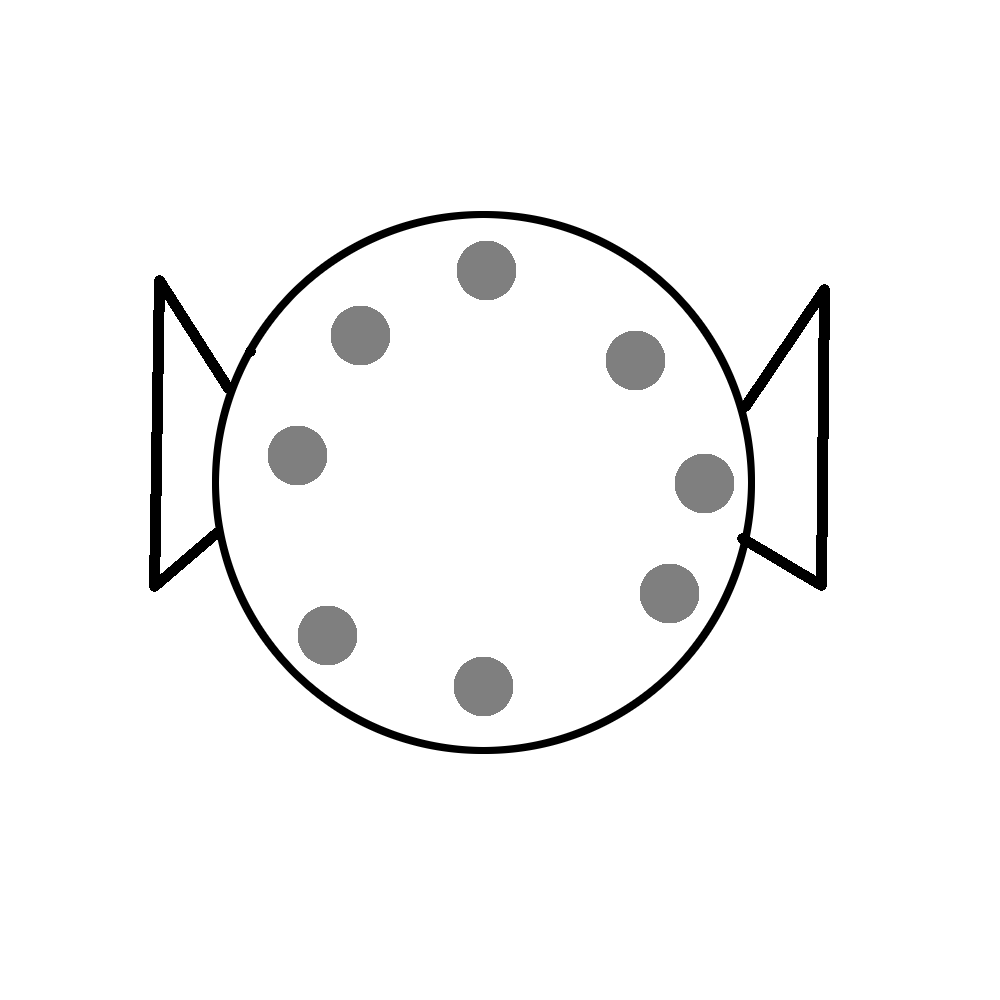
\includegraphics[width=.5\textwidth]{physic1}}%
	\only<2>{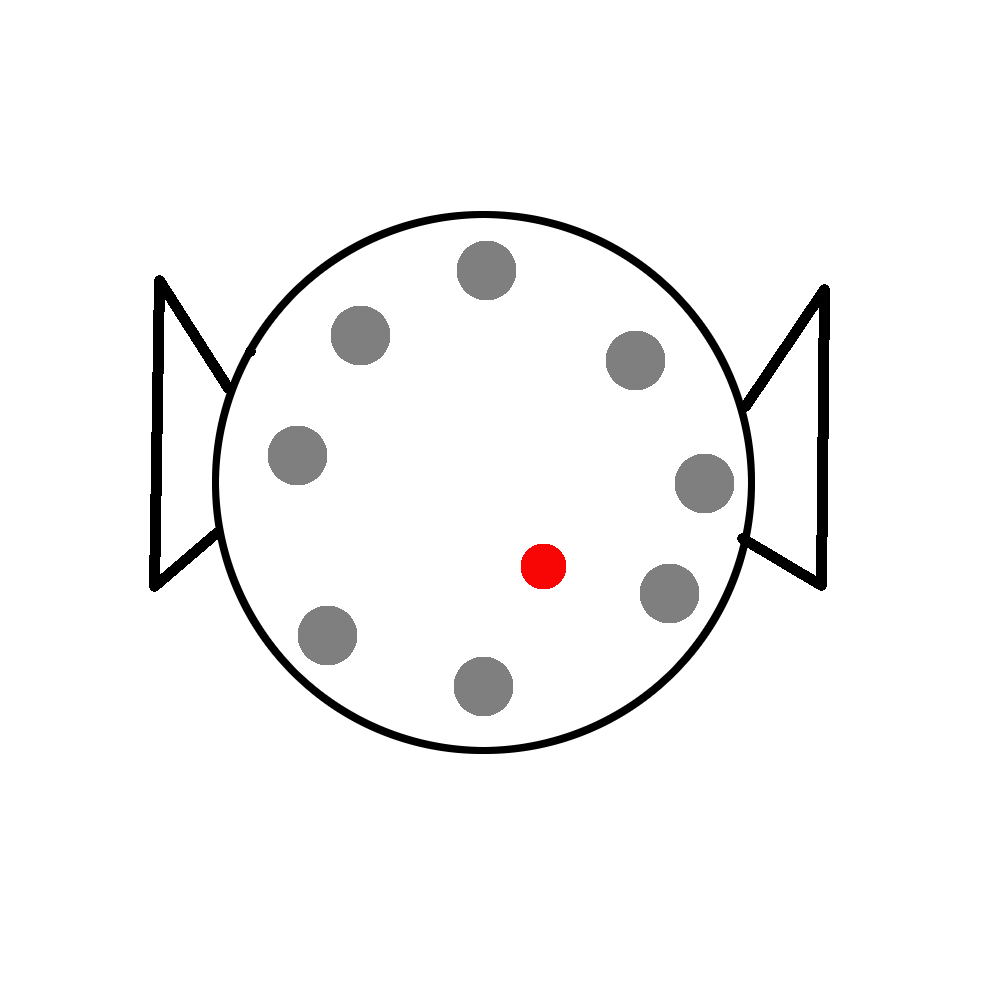
\includegraphics[width=.5\textwidth]{physic2}}%
	\only<3>{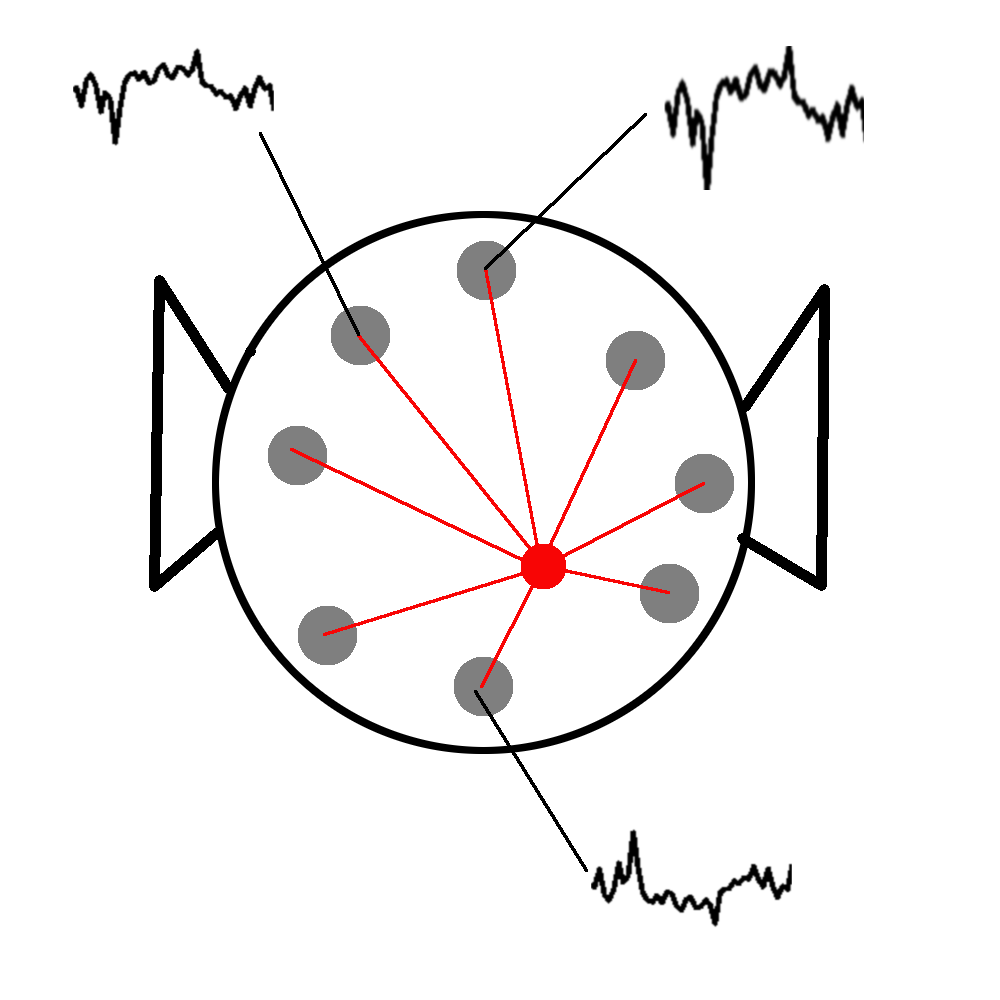
\includegraphics[width=.5\textwidth]{physic3}}
\end{frame}

\begin{frame}{Multivariate CSC with rank-1 constraint}
	\textbf{Idea}: Impose a rank-1 constraint on the dictionary atoms $D_k$
	\vskip1em
	To make the problem tractable, we decided to use auxiliary variables $u_k$ and $v_k$ \st{} $D_k = u_kv_k^\top$.

	\begin{equation}
	\label{eq:multichannel_csc}
	\begin{split}
	\min_{u_k, v_k, z_k^n} &\sum_{n=1}^N\frac{1}{2}\left\|X^n - \sum_{k=1}^K z^n_k * (u_k^{ } v_k^\top)\right\|_{2}^{2}
	+ \lambda  \sum_{k=1}^K \left\|z^n_k\right\|_1, \hspace{6pt}\\
	&\text{s.t. } ~~ \|u_{k}\|_2^2 \leq 1 \text{  , }\|v_{k}\|_2^2 \leq 1 \text{  and } z_k^n \geq 0~.
	\end{split}
	\end{equation}

	Here,
	\begin{itemize}
		\item $u_k \in \Rset^P$ is the spatial pattern of our atom
		\item $v_k \in \Rset^L$ is the temporal pattern of our atom
	\end{itemize}
\end{frame}

\begin{frame}{Optimization strategy}
\textbf{Tri-convex:} The problem is not jointly convex in $z^n_k$, $u_k$ and $v_k$ but it is convex in each block of coordinate.\\[1em]

We can use a block coordinate descent, aka alternate minimization, to converge to a local minima of this problem. The 3 following steps are applied alternatively:

\begin{itemize}
	\item \textbf{Z-step:} given a fixed estimate of the atom, compute the activation signal $z^n_k$ associated to each signal $X^n$.
	\item \textbf{u-step:} given a fixed estimate of the activation and temporal pattern, update the spatial pattern $u_k$.
	\item \textbf{v-step:} given a fixed estimate of the activation and spatial pattern, update the temporal pattern $v_k$.
\end{itemize}
\end{frame}

\begin{frame}{Z-step: Locally greedy coordinate descent (LGCD)}

$N$ independent problem such that
\[
	\label{eq:sparse_code}
	\min_{z_k^n \ge 0} \frac{1}{2} \left\|X^n - \sum_{k=1}^K z_k^n * D_k\right\|_2^2
	+ \lambda\sum_{k=1}^K\left\|z_k^n\right\|_1~.
\]
This problem is convex in $z_k$ and can be solved with different techniques:
\begin{itemize}
	\item Greedy CD \mycite{Kavukcuoglu2013}
	\item Fista \mycite{Chalasani2013}
	\item ADMM \mycite{Bristow2013}
	\item L-BFGS \mycite{Gramfort2017}
\end{itemize}

\strongpoint{These methods can be slow for long signals as the complexity of each iteration is at least linear in the length of the signal.}

\end{frame}

\begin{frame}[t]{Z-step: Locally greedy coordinate descent (LGCD)}

	For the Greedy Coordinate Descent, only 1 coordinate is updated at each iteration:
	\mycite{Kavukcuoglu2013}
	\vskip.5em
	\begin{enumerate}[<+->]\itemsep2em
		\item The coordinate $z_{k_0}[t_0]$ is updated to its optimal value $z'_{k_0}[t_0]$ when all other coordinate are fixed.
        \only<1>{
		\[
				z'_{k}[t] =  \max\left(\frac{\beta_{k}[t] - \lambda}{\| D_{k}\|_2^2}, 0\right) ,
		\]
		with $\beta_{k}[t] = \left[D_{k}^\Lsh * \left(X- \sum_{l=1}^K z_l * D_l +z_{k}[t]e_t* D_{k}\right)\right][t]$
        \vskip.5em
        For each coordinate update, it is possible to maintain the value of $\beta$ with $\mathcal O(KL)$ operations.
    }
		\item The updated coordinate is chosen
	\end{enumerate}

    \only<2>{
        \begin{itemize}
            \item Cyclic selection: $\mathcal{O}(1)$ \mycite{Friedman2007}
            \item Randomized selection: $\mathcal{O}(1)$ \mycite{Nesterov2010}
            \item Greedy selection: $\mathcal{O}(K\widetilde{T})$ \mycite{Osher2009}\\
            by maximizing $|z_k[t] - z'_k[t]|$
        \end{itemize}
    }

\end{frame}



\begin{frame}{Locally Greedy Coordinate Descent \mycite{Moreau2018}}


We introduced the LGCD method which is an extension of GCD.\\
{
    \centering
    \inputTikZ{.7}{tikz/LGCD}\\
}

\only<1-2>{
    \vskip1em
    GCD has $\mathcal O(K\widetilde{T})$ computational complexity.\\[1em]
    \only<2>{But the update itself has complexity $\mathcal O(KL)$}
}
%
\visible<3->{
    With a partition $\mathcal C_m$ of the signal domain $[1, K]\times [0, \widetilde{T}[$,
    \[
    \mathcal C_m = [1, K]\times [\frac{(m-1)\widetilde{T}}{M}, \frac{m\widetilde{T}}{M}[
    \]%
}%
\visible<4->{%
    The coordinate to update is chosen greedily on a sub-domain $\mathcal C_m$\\[1em]

    {\centering$\frac{\widetilde{T}}{M} = 2L-1~~\Rightarrow~~\mathcal O$(Coordinate selection) = $\mathcal O$(Coordinate Update)\\[1em]}

    The overall iteration complexity is $\mathcal O(KL)$ instead of $\mathcal O(K\widetilde{T})$.
    \begin{columns}
        \column{.5\textwidth}
        \strongpoint{Efficient for sparse $Z$}
        \column{.5\textwidth}
        \visible<5->{
        \strongpoint{Can be efficiently parallelized.}
        }
    \end{columns}
}


\end{frame}



\begin{frame}{D-step: solving for the atoms}

The dictionary update is performed by minimizing
\begin{equation}
\min_{\|D_k\|_2 \leq 1} E(D) \overset{\Delta}{=} \sum_{n=1}^N\frac{1}{2}\|X^n - \sum_{k=1}^K z^n_k * D_k\|_{2}^{2} \hspace{6pt}
\enspace .
\end{equation}

Computing $\nabla_{d_k} E(\{d_k\}_k)$ can be done efficiently
\[
\nabla_{D} E(D)
= \sum_{n=1}^N (z_k^n)^\Lsh * \left(x^n - \sum_{l=1}^K z^n_l * D_l\right)
=  \Phi_k - \sum_{l=1}^K \Psi_{k, l} *  D_l \enspace ,
\]

\strongpoint{Save with Projected Gradient Descent (PGD) with an Armijo backtracking line-search for the D-step \mycite{Wright1999}.}

\end{frame}


\begin{frame}{D-step: solving for the atoms}

	We use the projected gradient descent with an Armijo backtracking line-search \cite{Wright1999} for both u-step and v-step for
	\begin{equation}
		\begin{split}
			\min_{\substack{\|u_{k}\|_2 \leq 1\\\|v_{k}\|_2 \leq 1}} E(u_k, v_k) \overset{\Delta}{=} \sum_{n=1}^N\frac{1}{2}\|X^n - \sum_{k=1}^K z^n_k * (u_k^{ }  v_k^\top) \|_{2}^{2} \hspace{6pt}
			\enspace .
		\end{split}
	\end{equation}

	One important computation trick is for fast computation of the gradient.
	\[
	\begin{split}
		\nabla_{u_k} E(u_k, v_k) &=  \nabla_{D_k}E(u_k, v_k) v_k ~~ \in \Rset^{P}~,\\
		\nabla_{v_k} E(u_k, v_k) &=  u_k^\top \nabla_{D_k} E(u_k, v_k)  ~~ \in \Rset^L~,
	\end{split}
	\]
	Computing $\nabla_{D_k} E(u_k, v_k)$ can be done efficiently
	\[
	\nabla_{D_{k}} E(u_k, v_k) =  \sum_{n=1}^N (z_k^n)^\Lsh * \left(X^n - \sum_{l=1}^K z^n_l * D_l\right)
	=  \Phi_k - \sum_{l=1}^K \Psi_{k, l} *  D_l \enspace ,
	\]

\end{frame}

\section{Experiments}
\begin{frame}[t]
\vskip5em
\centering
\begin{beamercolorbox}[sep=8pt,center,shadow=true,rounded=true]{title}
	\usebeamerfont{title}\insertsectionhead%
\end{beamercolorbox}
\vskip5em
\flushleft
\large Good time to wake-up if you got lost in the previous section!
\end{frame}

\begin{frame}{Fast optimization}
    Comparison of the coordinate selection strategy for CD on simulated signals\\
    We set $K=10$, $L=150$, $\lambda = 0.1 \lambda_{\max}$\\[1em]
    \centering
    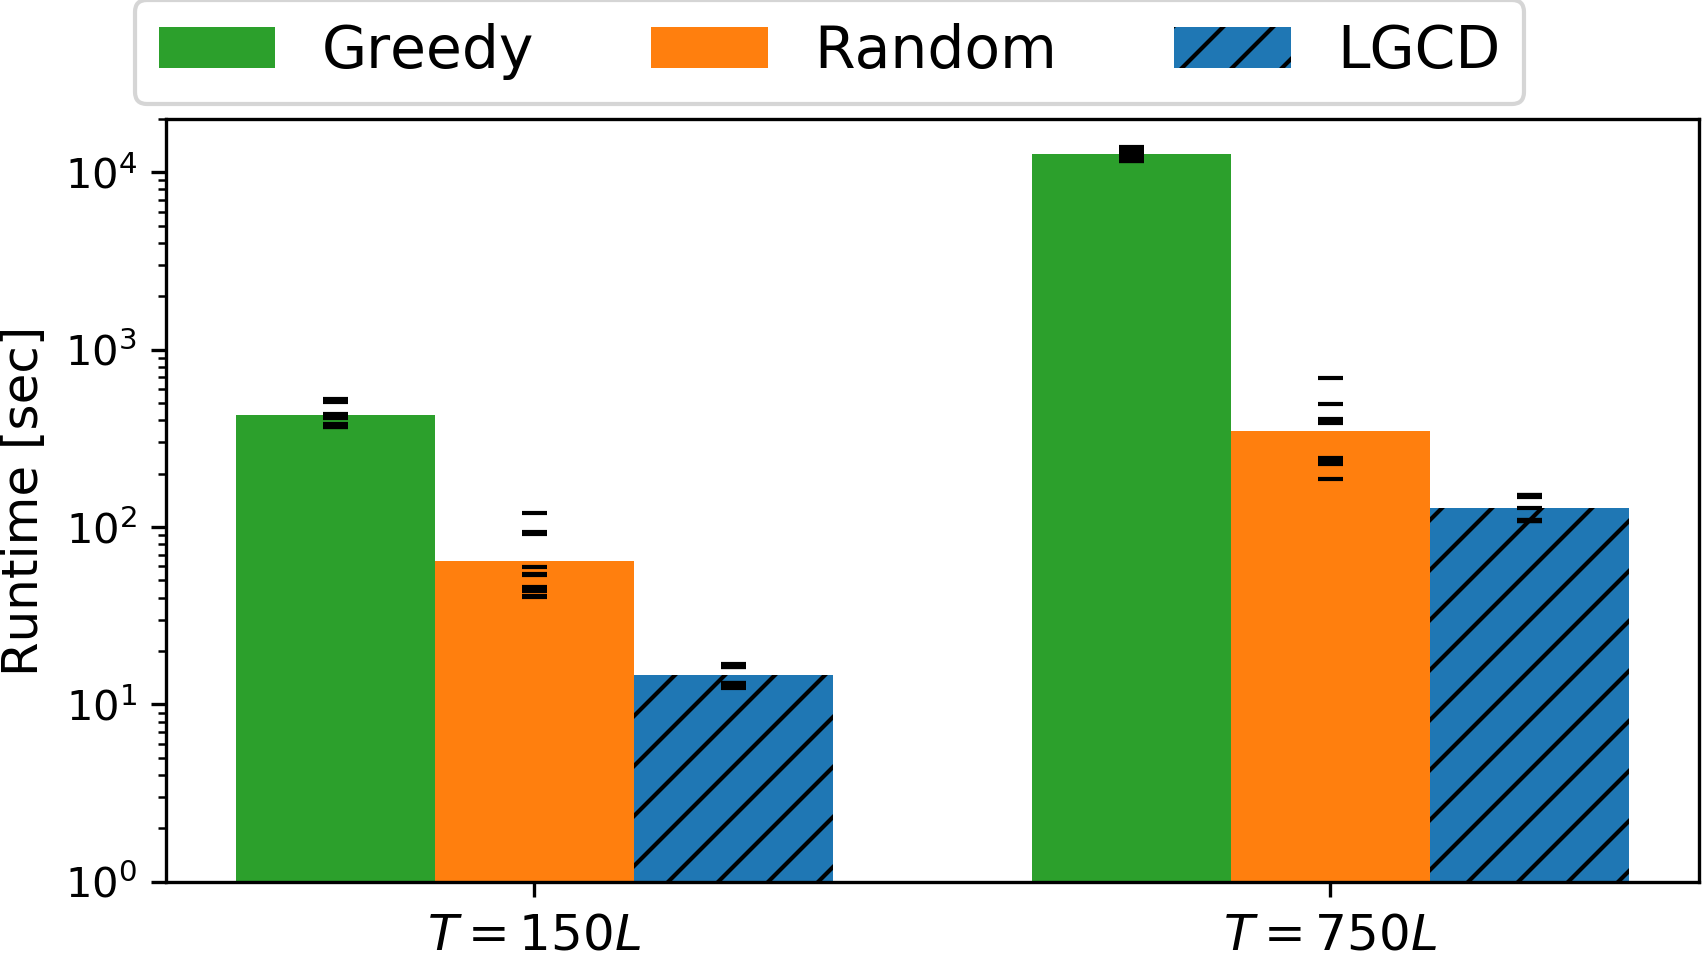
\includegraphics[width=.9\textwidth]{CD_strategies_comparison.png}
\end{frame}

\begin{frame}{Fast optimization}
Comparison with univariate methods on somato dataset with $T=134,700$, $K=8$ and $L=128$\\[1em]
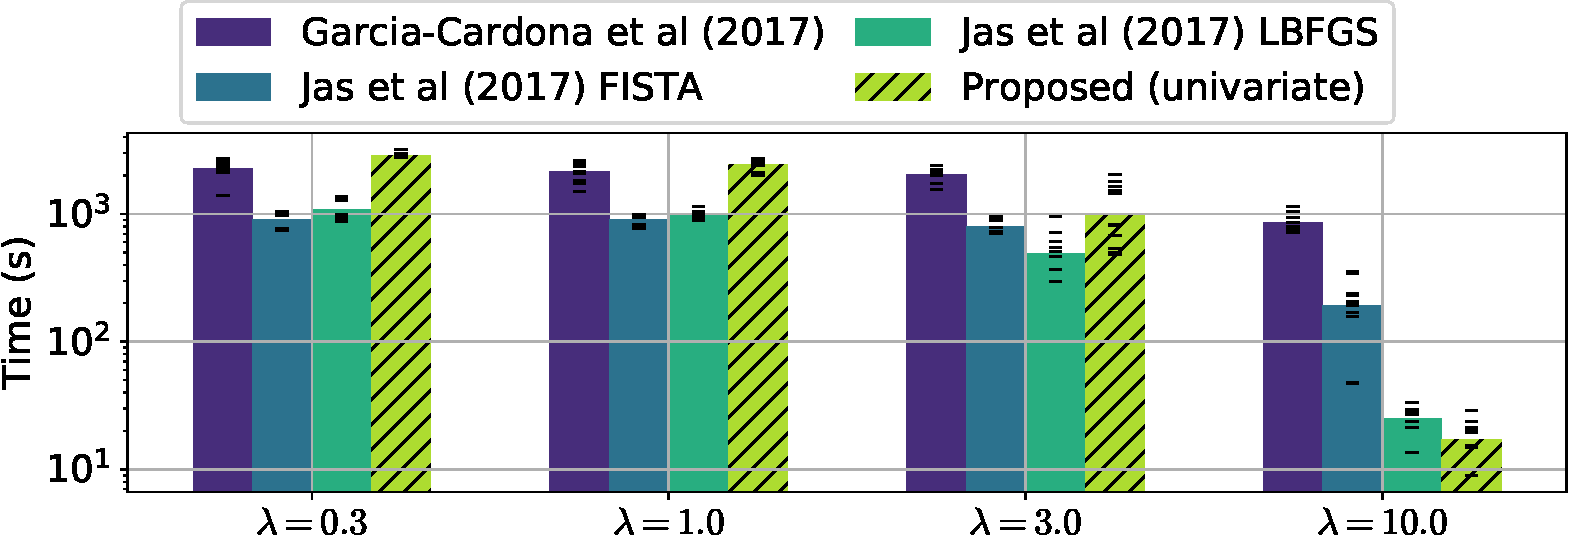
\includegraphics[width=\textwidth]{all_last_0001_T_13470_P1_K8_L128}
\end{frame}

\begin{frame}{Fast optimization}
Comparison with multivariate methods on somato dataset with $T=134,700$, $K=8$, $P=5$ and $L=128$\\[1em]
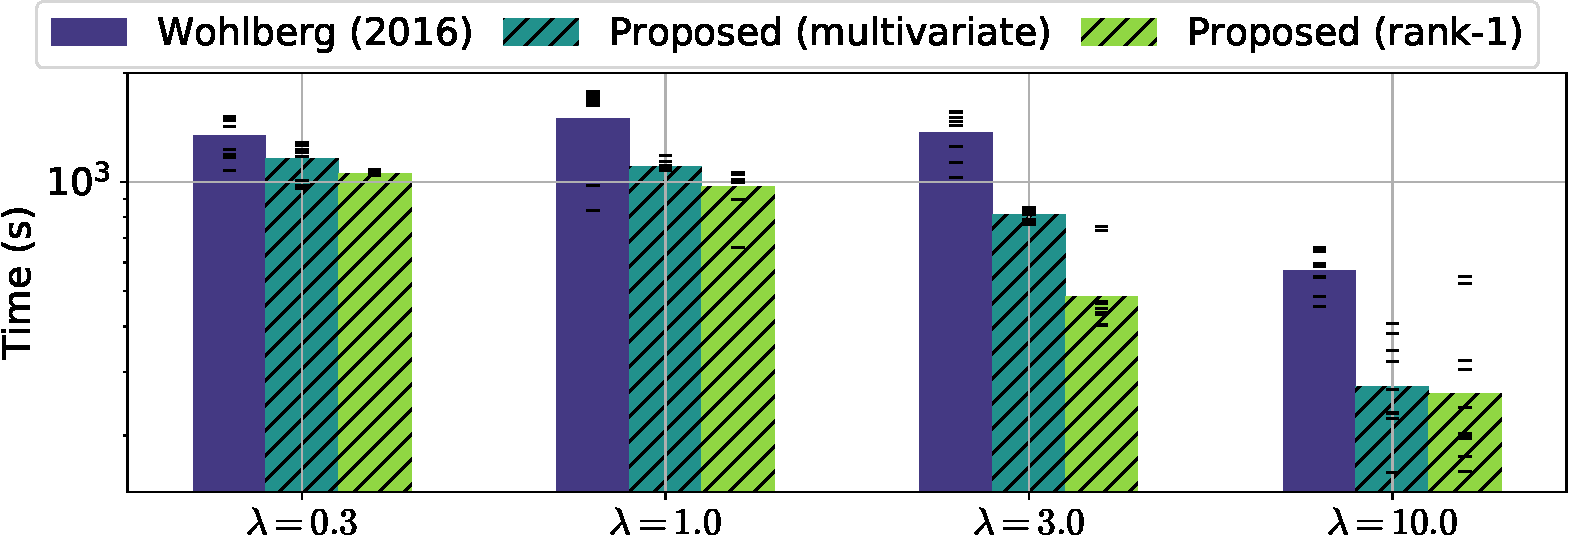
\includegraphics[width=\textwidth]{all_last_0001_T_13470_P5_K8_L128}
\end{frame}

\begin{frame}{Good scaling in the number of channels $P$}
Scaling relative to $P$ on somato dataset with $T=134,700$, $K=2$, and $L=128$\\[1em]
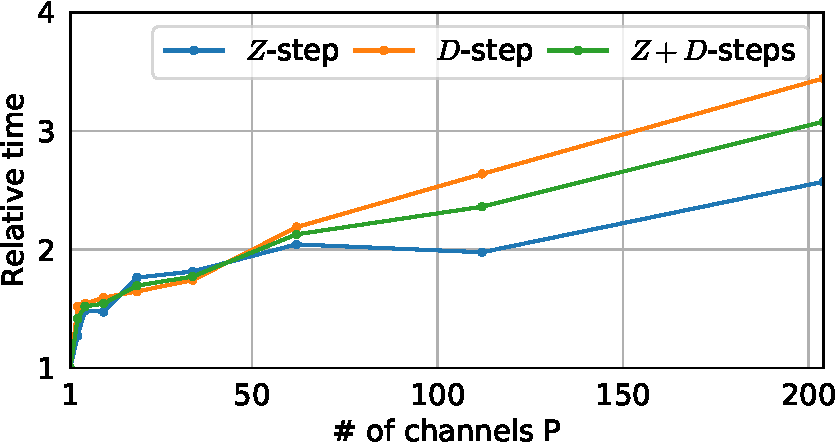
\includegraphics[width=\textwidth]{scaling_channels_reg0_001_mean_rank1_K2_L128.pdf}
\end{frame}

\begin{frame}{Pattern recovery}
Test the pattern recovery capabilities of our method on simulated data,
\[
	X^n = \sum_{k=1}^2 z_k * (u_kv_k^\top) + \mathcal E
\]
where $(u_k, v_k)$ are chosen patterns of rank-1 and the activated coefficient $z^n_k[t]$ are drawn uniformly and their value are uniform in $[0, 1]$.\\[1em]
The noise $\mathcal E$ is generated as a gaussian white noise with variance $\sigma$.\\[1em]

We set $N=100$, $L=64$ and $\tT=640$
\end{frame}

\begin{frame}{Pattern recovery}
Patterns recovered with $P = 1$ and $P=5$. The signals were generated with the two simulated temporal patterns and with  $\sigma = 10^{-3}$. \\[1em]
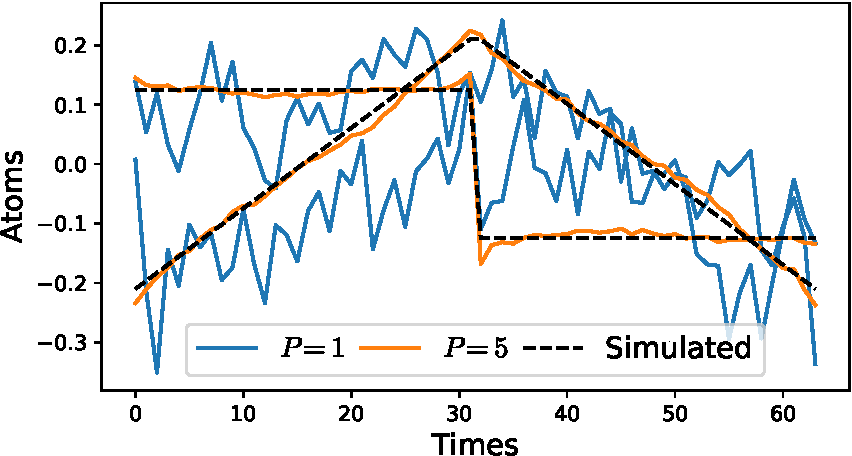
\includegraphics[width=\textwidth]{1D_vs_multi_uv_hat_P5.pdf}
\end{frame}
\begin{frame}{Pattern recovery}
Evolution of the recovery loss with $\sigma$ for different values of $P$. Using more channels improves the recovery of the original patterns.\\[1em]
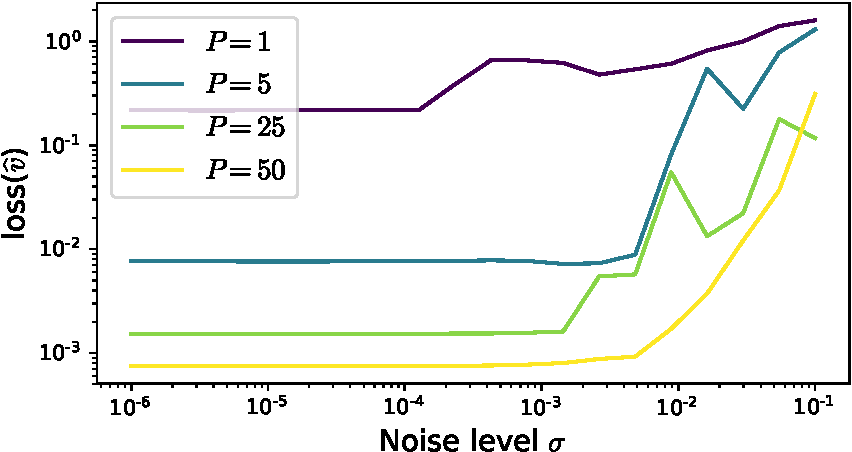
\includegraphics[width=\textwidth]{1D_vs_multi.pdf}
\end{frame}


\section{Experiments on MEG data}
\begin{frame}[t]
\vskip5em
\centering
\begin{beamercolorbox}[sep=8pt,center,shadow=true,rounded=true]{title}
	\usebeamerfont{title}\insertsectionhead%
\end{beamercolorbox}
\vskip5em
\flushleft
\large Even better time to wake-up!
\end{frame}

\begin{frame}{MNE somatosensory data}
A selection of temporal waveforms of the atoms learned on the MNE sample dataset.\\[1em]
\centering
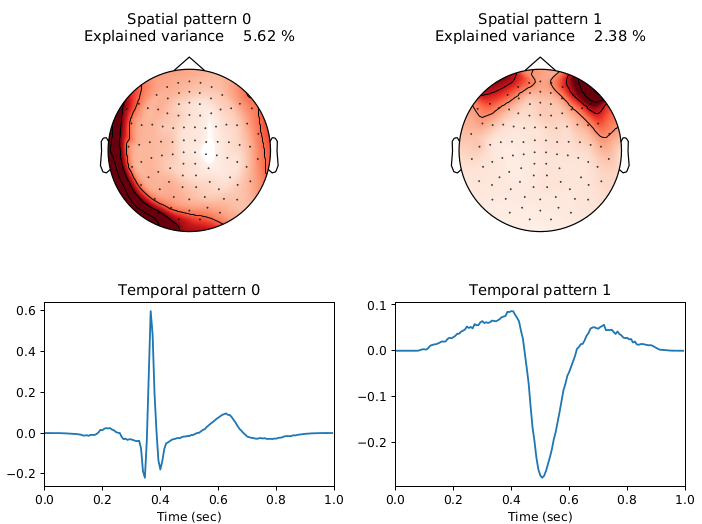
\includegraphics[height=0.7\textheight]{artifacts}
\end{frame}


\frame[t]{
    \frametitle{Learned atoms -- Evoked response}

    \centering
    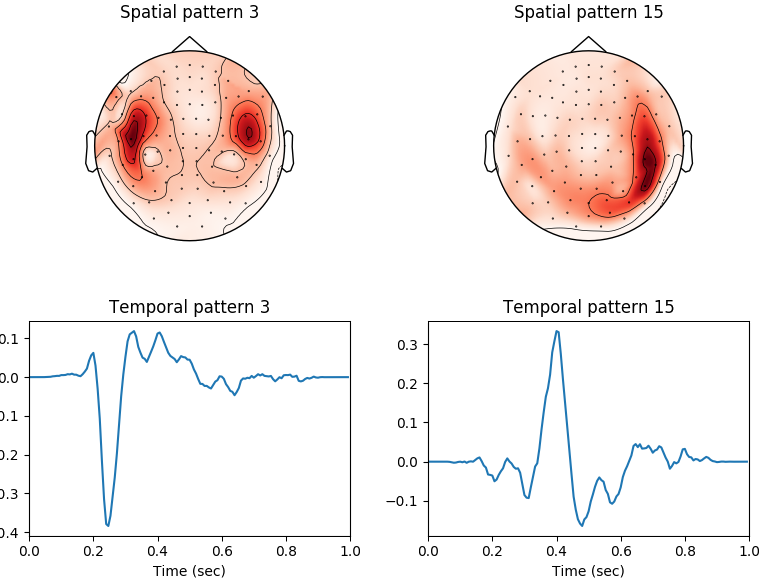
\includegraphics[width=.9\columnwidth]{evoked}
}


\frame[t]{
    \frametitle{Learned atoms -- Evoked response}

    \centering
    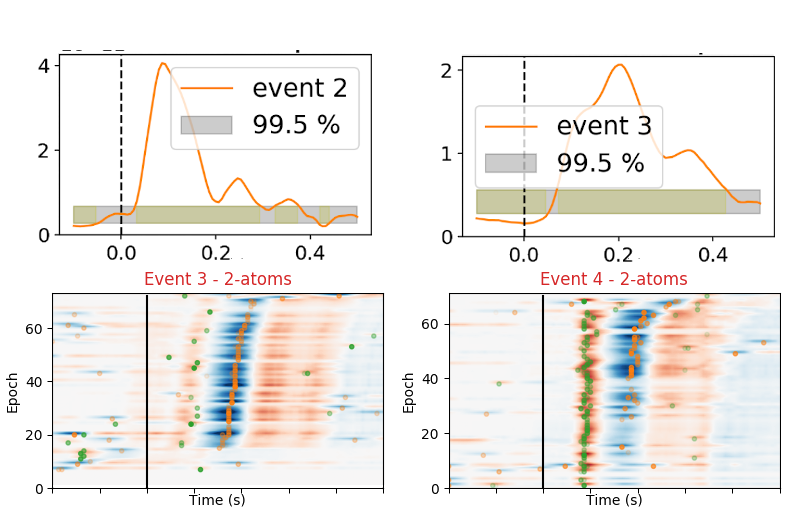
\includegraphics[width=.9\columnwidth]{activations}
    \vskip-12em
    \visible<2>{
    \begin{columns}
        \column{.4\columnwidth}
        \highlightbox{\centering \Huge Work in progress!}
    \end{columns}
    }

}
\frame[t]{
    \frametitle{Learned atoms -- Complex waveforms}

    \centering
    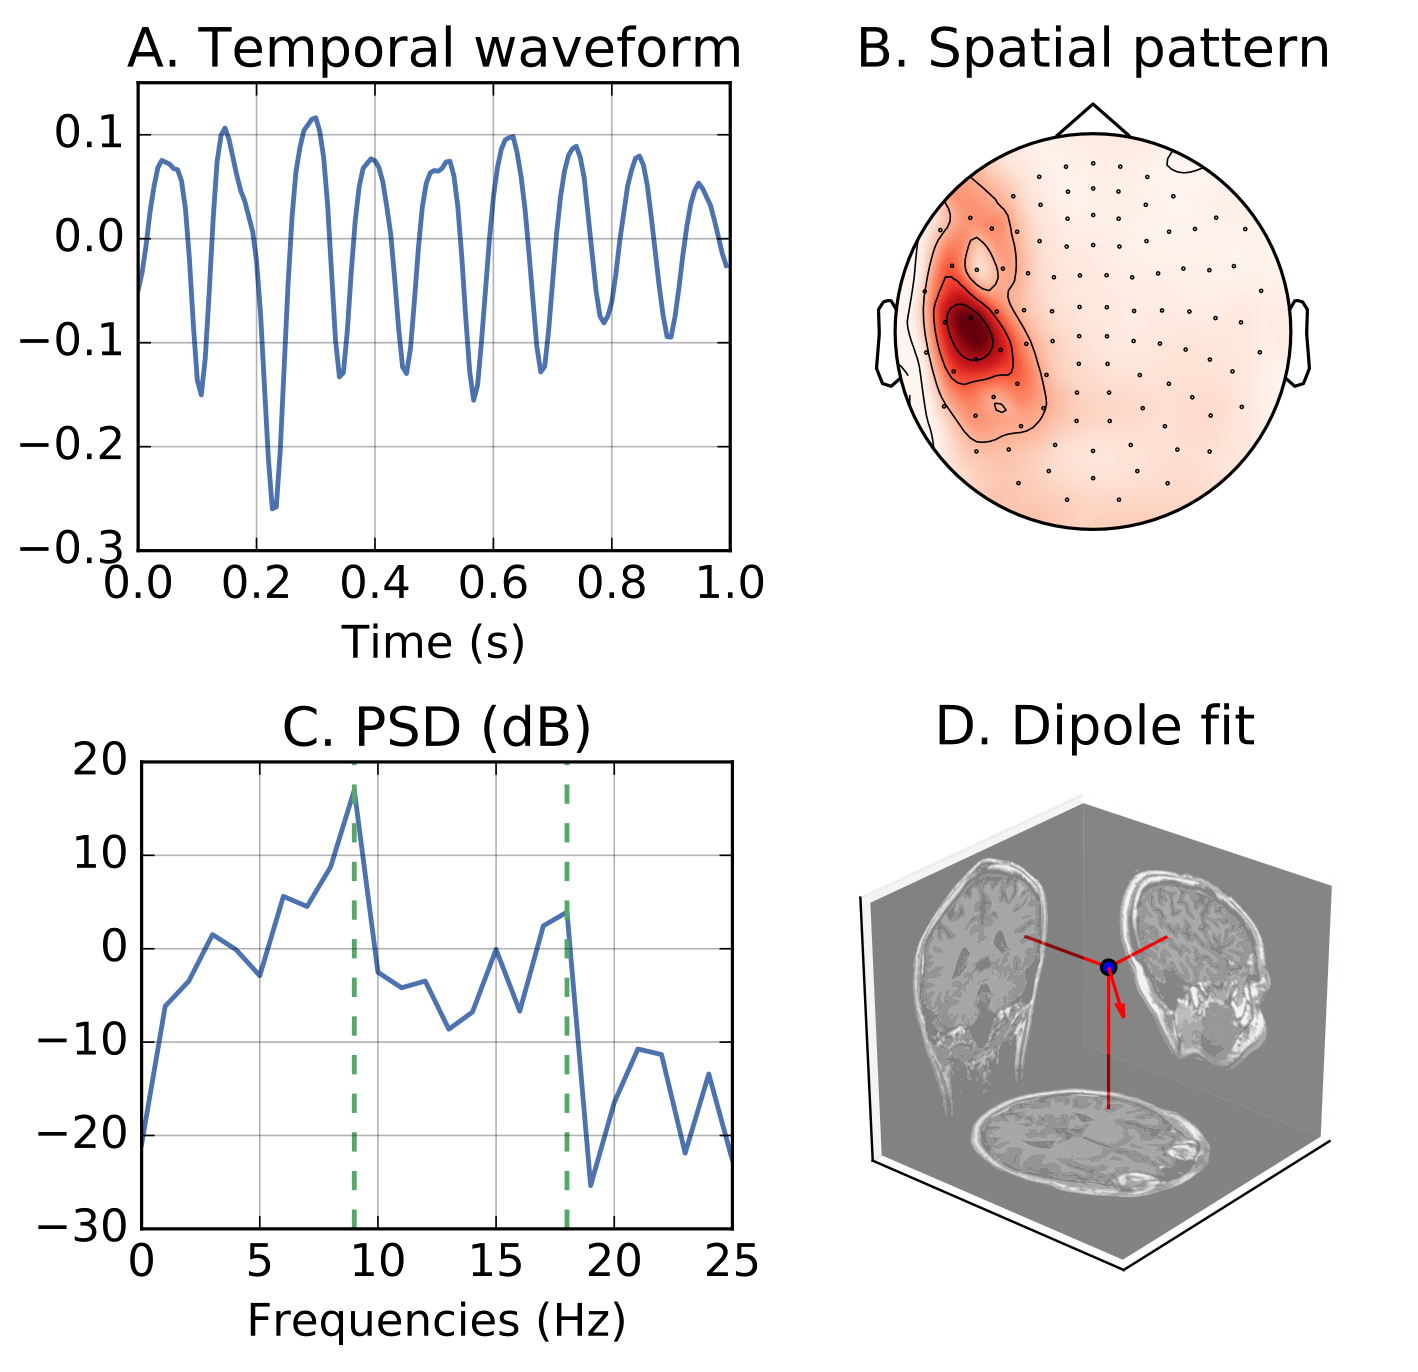
\includegraphics[width=.7\columnwidth]{atom_somato}
}

{\usebackgroundtemplate{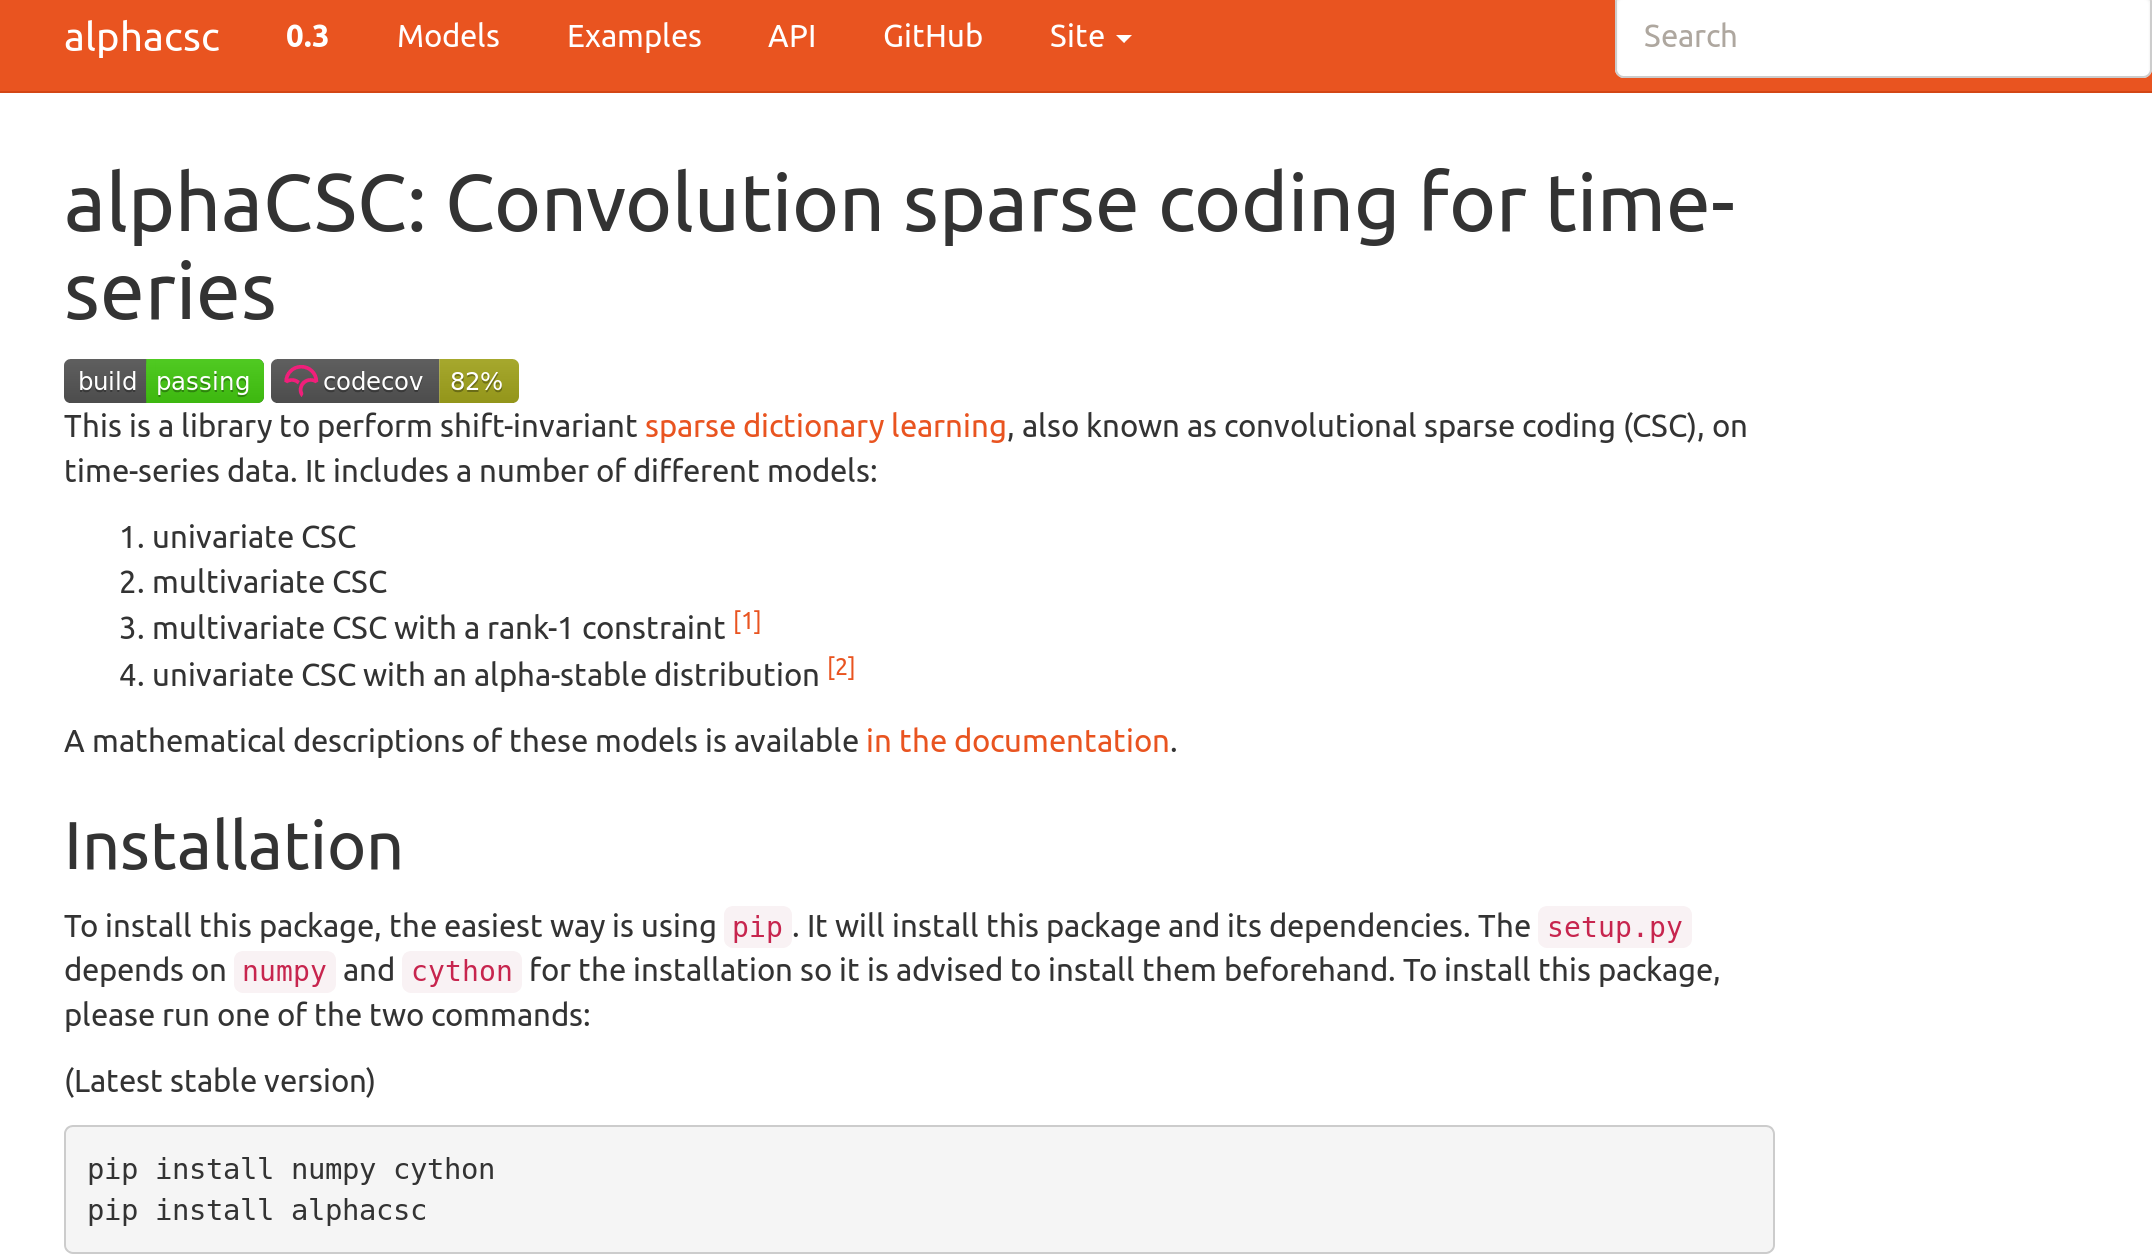
\includegraphics[width=\paperwidth]{alphacsc}}%
\frame{
    \begin{columns}
        \column{.5\textwidth}
        \column{.4\textwidth}
        \highlightbox{Python code online:\\
                        https://alphacsc.github.io\\[1em]
                        \texttt{pip install alphacsc}}
        \vskip2em
            \highlightbox{Examples reproduce figures from this talk!}

    \end{columns}
}}


\begin{frame}{}
\vskip2em
{\centering
    \usebeamercolor[fg]{title}
    \usebeamerfont{title}
    \Huge \bf Thanks for your attention!\\[2em]}

Code available online:\\[1em]


\includegraphics[height=.8em]{github}~\textbf{alphacsc} :  alphacsc.github.io\\[1em]

\includegraphics[height=.8em]{github}~\textbf{DiCoDiLe} : github.com/tommoral/dicodile\\[2em]

Slides are on my web page:\\[1em]
\hskip5em\includegraphics[height=.8em]{website} tommoral.github.io
\hskip4em 
\includegraphics[height=.8em]{twitter} @tomamoral


\end{frame}

\end{document}
